\section{Quantum Dots}

The focus regarding quantum dots has been on studying the distribution of electrons as a function of the level of confinement. In addition, ground state energies are provided and compared to other many-body methods to demonstrate the efficiency and precision of Variational Monte-Carlo (VMC) and Diffusion Monte-Carlo (DMC). In the case of two dimensional quantum dots, there are multiple published results, however, for three dimensions this is not the case. An introduction to quantum dots is given in Section \ref{sec:modelQDots}. 

The double-well quantum dot has not been a focus in this thesis, however, some simple results are provided to demonstrate the flexibility of the code.

\subsection{Ground State Energies}

\subsubsection{Two dimensional quantum dots}

Table \ref{tab:QDotsResultsAll} presents the calculated ground state energies for two-dimensional quantum dots in addition to corresponding results from methods such as Similarity Renormalization Group theory (SRG), Coupled Cluster Singles and Doubles (CCSD) and Full Configuration Interaction (FCI). In addition, some previously published DMC results are supplied. The references are listed in the table caption.

In light of the variational nature of DMC and VMC, the results show that DMC provides a more precise estimate for the ground state energy than VMC, both in terms of lower energies and lower errors. The exact energy in the case of two electrons with $\omega=1$ has been calculated in Ref. \cite{taut} and is $E_0 = 3$, which is in excellent agreement with the presented results.

The DMC energies calculated in this thesis has a lower error than those provided in Ref. \cite{MagnusArticle}. This may only be due to the fact that the calculations in this thesis have been run on a super computer. Running smaller simulations on fewer processors results in larger errors. Both the implementations successfully agree with the FCI result for two particles, which strongly indicates that the disagreements in results are a result of systematic errors.    

In the case of two particles, DMC and FCI agree up to five decimals, which leads to the conclusion that DMC indeed is a very precise method. The SRG method is not variational in the sense that it can undershoot the exact energy. The DMC result should thus not be read as less precise in the cases where SRG provides a lower energy estimate. Diffusion Monte-Carlo and SRG are in excellent agreement for a large number of particles compared to FCI and CCSD, which drift away from the DMC results as their basis sizes shrink. 

For high frequencies, the VMC energy is higher than the CCSD energy. The fact that both the methods are variational implies that CCSD performs better than VMC in this frequency range. However, looking at the results the lower frequency range, it is clear that VMC performs better than CCSD. This is due to the fact that CCSD struggles with convergence as the correlations within the system increase, indicated by the decrease in number of shells used to perform the calculations.

The DMC energy is overall less than the CCSD energy, which, due to the variational nature of the methods, implies that DMC performs better than CCSD. The results for $56$ particles are in excellent agreement with each other. 

\setlength{\tabcolsep}{5pt}
\begin{table}
\begin{center}
\begin{tabular}{cc|rrrrrr}
    N     & $\omega$ & $\mathrm{E_{VMC}}$ & $\mathrm{E_{DMC}}$ & $E_\mathrm{ref}^{(a)}$& $E_\mathrm{ref}^{(b)}$ & $E_\mathrm{ref}^{(c)}$ & $E_\mathrm{ref}^{(d)}$\\
\hline\hline
\multicolumn{8}{c}{} \\
    2     &   0.01   & 0.07406(5)  & 0.073839(2)  & -		& -			& 0.0738 \{23\} & 0.07383505 \{19\}\\
          &   0.1    & 0.44130(5)  & 0.44079(1)   & - 		& - 			& 0.4408 \{23\} & 0.44079191 \{19\}\\
          &   0.28   & 1.02215(5)  & 1.02164(1)   & -		&0.99263 \{19\} 	& 1.0217 \{23\}  & 1.0216441 \{19\}\\
          &   0.5    & 1.66021(5)  & 1.65977(1)   & 1.65975(2)&1.643871 \{19\}	& 1.6599 \{23\}  & 1.6597723 \{19\}\\
          &   1.0    & 3.00030(5)  & 3.00000(1)   & 3.00000(3)&2.9902683 \{19\}	& 3.0002 \{23\}  & 3.0000001 \{19\}\\
\cline{2-8}
\multicolumn{8}{c}{} \\
    6     &   0.1    &  3.5690(3)  &  3.55385(5)  & -		&3.49991 \{18\} 	& 3.5805 \{22\}  & 3.551776 \{9\}\\
          &   0.28   &  7.6216(4)  &  7.60019(6)  & 7.6001(1) &7.56972 \{18\} 	& 7.6254 \{22\}  & 7.599579 \{6\}\\
          &   0.5    & 11.8103(4)  & 11.78484(6)  & 11.7888(2)&11.76228 \{18\}	& 11.8055 \{22\} & 11.785915 \{6\}\\
          &   1.0    & 20.1902(4)  & 20.15932(8)  & 20.1597(2)&20.14393 \{18\}	& 20.1734 \{22\} & 20.160472 \{8\}\\
\cline{2-8}
\multicolumn{8}{c}{} \\
    12    &   0.1    & 12.3162(5)  & 12.26984(8)  & - 		&12.2253 \{17\} 	& 12.3497 \{21\} & 12.850344 \{3\}\\
          &   0.28   & 25.7015(6)  & 25.63577(9)  & - 		&25.61084 \{17\} 	& 25.7095 \{21\} & 26.482570 \{2\}\\
          &   0.5    & 39.2343(6)  & 39.1596(1)   & 39.159(1) &39.13899 \{17\}	& 39.2194 \{21\} & 39.922693 \{2\}\\
          &   1.0    & 65.7905(7)  & 65.7001(1)   & 65.700(1) &65.68304 \{17\}	& 65.7399 \{21\} & 66.076116 \{3\}\\
\cline{2-8}
\multicolumn{8}{c}{} \\
    20    &   0.1    &  30.0729(8)  &  29.9779(1) & -		&29.95345 \{16\}	& 30.2700 \{8\} & 34.204867 \{1\}\\
          &   0.28   &  62.0543(8)  &  61.9268(1) & 61.922(2) &61.91368 \{16\}	& 62.0676 \{20\} & 67.767987 \{1\}\\
          &   0.5    &  94.0236(9)  &  93.8752(1) & 93.867(3) &93.86145 \{16\}	& 93.9889 \{20\} & 100.93607 \{1\}\\
          &   1.0    & 156.062(1)   & 155.8822(1) & 155.868(6)&155.8665 \{16\}	& 155.9569 \{20\}& 164.61280 \{1\}\\
\cline{2-8}
\multicolumn{8}{c}{} \\
    30    &   0.1    &  60.584(1)  &  60.4205(2)  & -		&60.43000 \{15\}	&  61.3827 \{9\}& -\\
          &   0.28   & 124.181(1)  & 123.9683(2)  & - 		&123.9733 \{15\}	& 124.2111 \{9\}& -\\
          &   0.5    & 187.294(1)  & 187.0426(2)  & - 		&187.0408 \{15\}	& 187.2231 \{19\}& -\\
          &   1.0    & 308.858(1)  & 308.5627(2)  & -	 	&308.5536 \{15\}	& 308.6810 \{19\}& -\\
\cline{2-8}
\multicolumn{8}{c}{} \\
    42    &   0.1    & 107.881(1)  & 107.6389(2)  & - 		&- 			& 111.7170 \{8\}& -\\
          &   0.28   & 220.161(1)  & 219.8426(2)  & - 		&219.8836 \{14\}	& 222.1401 \{8\}& -\\
          &   0.5    & 331.002(1)  & 330.6306(2)  & - 		&330.6485 \{14\}	& 331.8901 \{8\}& -\\
          &   1.0    & 544.2(8)    & 542.9428(8)  & - 		&542.9528 \{14\}	& 543.1155 \{18\}& -\\
\cline{2-8}
\multicolumn{8}{c}{} \\
    56    &   0.1    & 176.269(2) & 175.9553(7)   & -		& -		& 186.1034 \{9\} & -		\\
          &   0.28   & 358.594(2) & 358.145(2)    & -		& -		& 363.2048 \{9\} & -		\\
          &   0.5    & 538.5(6)   & 537.353(2)    & -		& -		& 540.3430 \{9\} & -		\\
          &   1      & 880.2(7)   & 879.3986(6)   & -		& -		& 879.6386 \{17\}& -		\\
\hline\hline


\end{tabular}
\caption{Ground state energy results for two dimensional $N$-electron quantum dots with frequency $\omega$. Refs. $(a)$: F. Pederiva \cite{MagnusArticle} (DMC), $(b)$: S. Reimann \cite{Sarah} (Similarity Renormalization Group theory), $(c)$: C. Hirth \cite{Hirth} (Coupled Cluster Singles and Doubles), $(d)$: V. K. B. Olsen \cite{Olsen} (Full Configuration Interaction). The numbers inside curly brackets denote the number of shells used above \textit{Fermi-level} to construct the basis for the corresponding methods.}
\label{tab:QDotsResultsAll}
\end{center}
\end{table}
\setlength{\tabcolsep}{6pt}


\clearpage
\subsubsection{Three dimensional quantum dots}

\setlength{\tabcolsep}{1.05cm}
\begin{table}
\begin{center}
\begin{tabular}{cc|rrr}
    N     & $\omega$ & $\mathrm{E_{VMC}}$ & $\mathrm{E_{DMC}}$ & $E_\mathrm{ref}$\\
\hline\hline
\multicolumn{5}{c}{} \\
    2     &   0.01   & 0.07939(3)  & 0.079206(3) & -		\\
          &   0.1    & 0.50024(8)  & 0.499997(3) & 0.5        \\
          &   0.28   & 1.20173(5)  & 1.201725(2) & -		\\
          &   0.5    & 2.00005(2)  & 2.000000(2) & 2.0 \\
          &   1.0    & 3.73032(8)  & 3.730123(3) & - \\
\cline{2-5}
\multicolumn{5}{c}{} \\
    8     &   0.1    & 5.7130(6)   & 5.7028(1)   & - 		\\
          &   0.28   & 12.2040(8)  & 12.1927(1)  & -		\\
          &   0.5    & 18.9750(7)  & 18.9611(1)  & -\\
          &   1.0    & 32.6842(8)  & 32.6680(1)  & -\\
\cline{2-5}
\multicolumn{5}{c}{} \\
    20    &   0.1    & 27.316(2)   & 27.2717(2)   & - 		\\
          &   0.28   & 56.440(2)   & 56.3868(2)   & -		\\
          &   0.5    & 85.714(2)   & 85.6555(2)   & - \\
          &   1.0    & 142.951(2)  & 142.8875(2)  & -\\
\cline{2-5}
\multicolumn{5}{c}{} \\
\hline\hline
\end{tabular}
\caption{Ground state energy results for three-dimensional $N$-electron quantum dots with frequency $\omega$. The values in the fifth column is exact calculations taken from Ref. \cite{taut}. The VMC result is as expected always higher than the corresponding DMC result.}
\label{tab:QDotsResults3D}
\end{center}
\end{table}
\setlength{\tabcolsep}{6pt}

The results for three dimensional quantum dots are presented in Table \ref{tab:QDotsResults3D}. Three dimensional quantum dots do not have the same foothold in literature as the two dimensional ones, hence no results are listed except for some exact solutions taken from Ref. \cite{taut}. 

As expected, DMC reproduces the exact results for two particles. Compared to the exact results for two dimensions, which was reproduced with five digit precision, the exact results are reproduced with six decimal precision for three dimensions. This strongly indicates that for two electrons, DMC behaves better for three dimensions than for two. For higher number of particles, however, the errors are of the same order of magnitude as for two dimensions, leading to the conclusion that DMC performs equally good in either dimension for quantum dots. 

\subsection{One-body Densities}

The one-body densities are calculated using the methods described in Section \ref{sec:OBD}.

Figure \ref{fig:OBD_DMC_QDOTS_w1} presents the one-body densities for two-dimensional quantum dots. It is clear that the distribution is following a clear trend: Odd number of closed shells ($N=2$, 12, 30) are all similar in shape. It is almost as if the $N=2$ case is a zoom-in of the $N=12$ top, which in turn is a zoom-in of the $N=30$ top. A physical explanation is that the shapes are conserved due to the fact that they represent energetically favorable configurations. 

The same trend is present for the even numbered shells ($N=6$, 20, 42) as well. The density for $N=56$, which is not included in the figure, further demonstrates this trend. Viewing the distributions as a sequence of images, from the lowest number of particles to the highest, it is apparent that the shape propagates very much like water ripples. It is remarkable how the solutions to the most complex of equations can come in the form of simple patterns found all around nature.


\clearpage
\captionsetup[subfloat]{labelformat=empty}
\begin{figure}
 \begin{center}
  \subfigure[$N=2$]{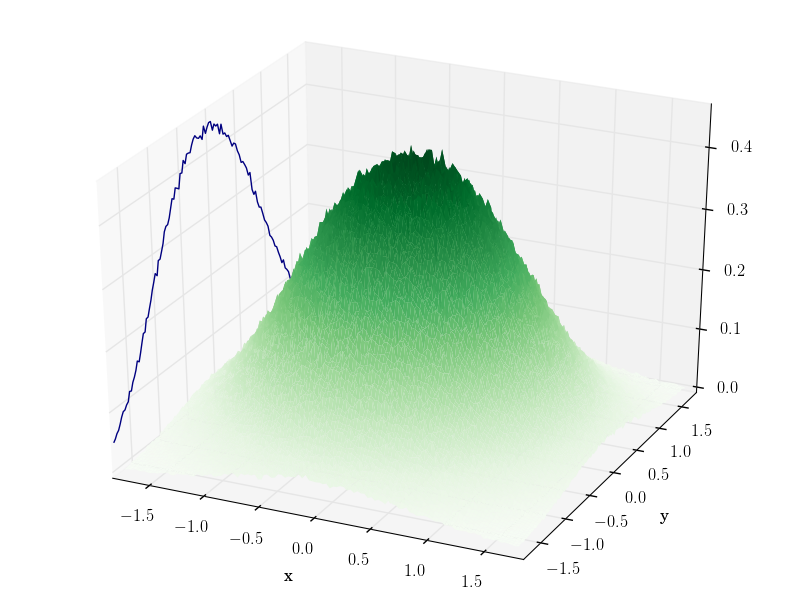
\includegraphics[scale=0.35]{../Graphics/OBD/OBD_DMC/dist_out_QDots2c1_3D.png}}
  \subfigure[$N=6$]{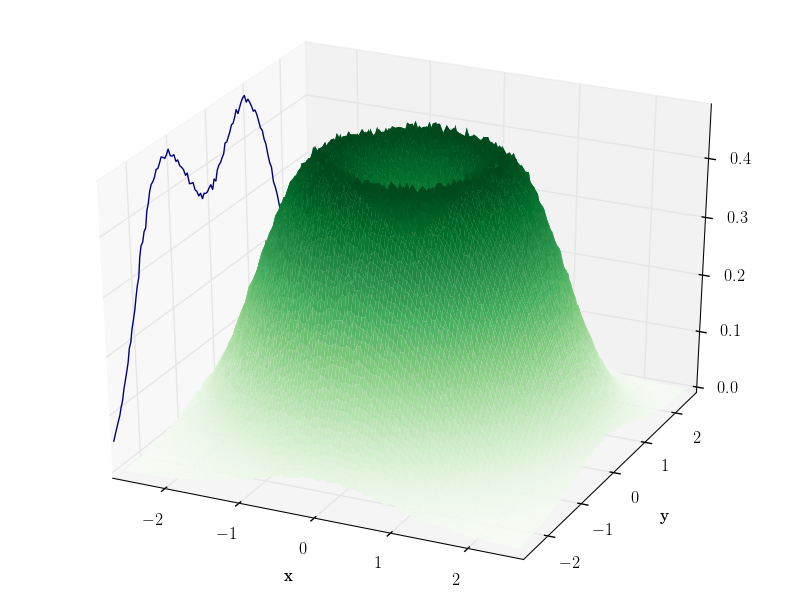
\includegraphics[scale=0.35]{../Graphics/OBD/OBD_DMC/dist_out_QDots6c1_3D.png}} \\
  \subfigure[$N=12$]{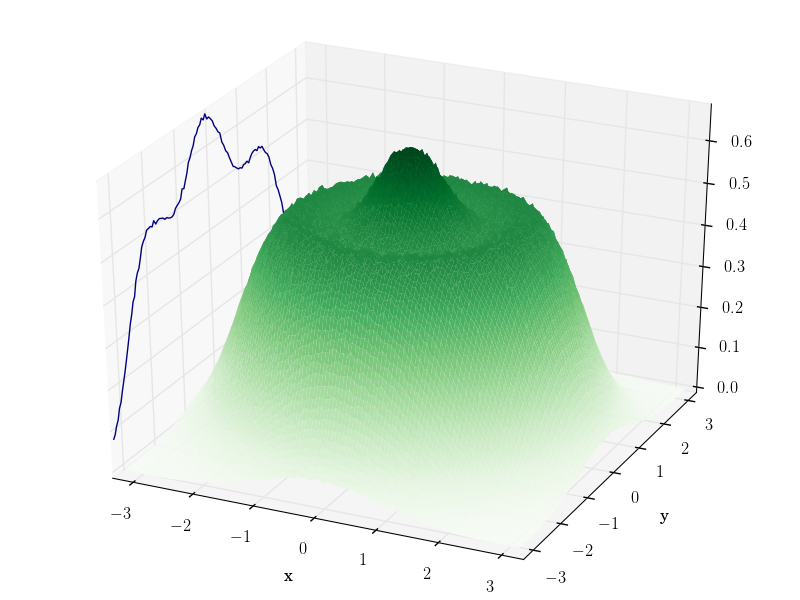
\includegraphics[scale=0.35]{../Graphics/OBD/OBD_DMC/dist_out_QDots12c1_3D.png}}
  \subfigure[$N=20$]{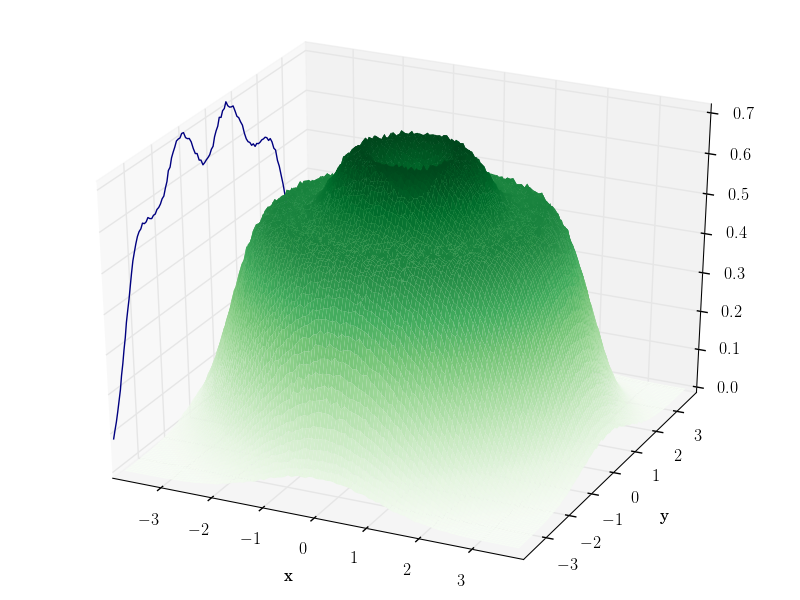
\includegraphics[scale=0.35]{../Graphics/OBD/OBD_DMC/dist_out_QDots20c1_3D.png}} \\
  \subfigure[$N=30$]{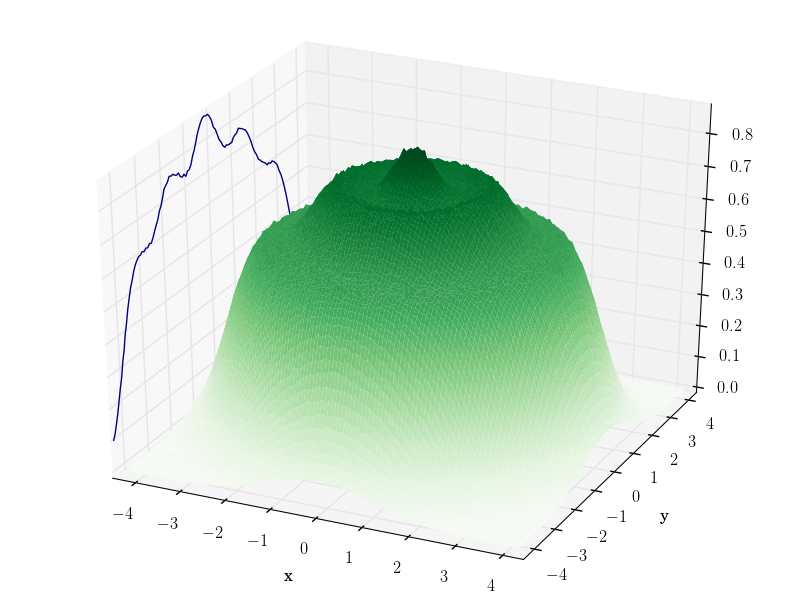
\includegraphics[scale=0.35]{../Graphics/OBD/OBD_DMC/dist_out_QDots30c1_3D.png}}
  \subfigure[$N=42$]{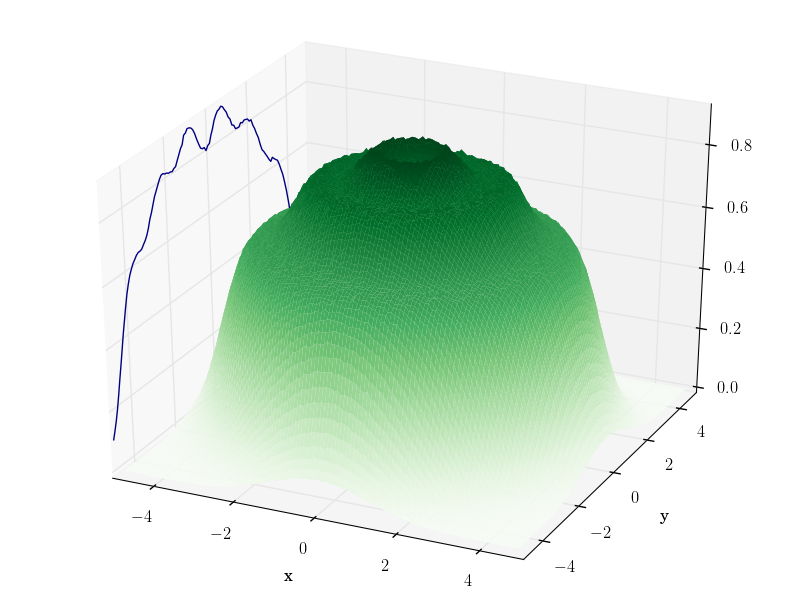
\includegraphics[scale=0.35]{../Graphics/OBD/OBD_DMC/dist_out_QDots42c1_3D.png}} \\
  \caption{Diffusion Monte-Carlo one-body densities for two dimensional quantum dots with frequency $\omega=1$. The number of particles $N$ are listed below each density. It is apparent that the density behaves much like water ripples as the number of particles increase, conserving the shape in an oscillatory manner.}
  \label{fig:OBD_DMC_QDOTS_w1} 
 \end{center}
\end{figure}

\clearpage

 Adding a third positional dimension changes the shape of the Schrödinger equation, which due to the Coulomb interaction is not separable in Cartesian coordinates. In other words, by going to three dimensions, the general shape of the solutions are expected to change. Nevertheless, by looking at the one-body densities for three dimensions in Figure \ref{fig:OBD_QDOTS3D_highfreq}, it is apparent that the general density profile is unchanged with respect to the number of closed shells. However, by comparing the two dimensional density for $N=20$ electrons from Figure \ref{fig:OBD_DMC_QDOTS_w1} with the three dimensional one for the same number of particles, it is clear that the shape of the densities are not conserved with respect to $N$ alone.

% \setlength{\tabcolsep}{0.1pt}
\begin{figure}
 \begin{center}
 \begin{tabular}{cc|c}
   \subfigure{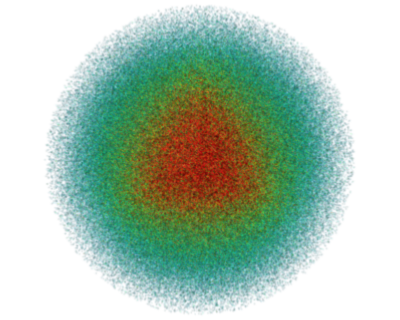
\includegraphics[scale=0.3]{../Graphics/OBD/OBD_Q3D/QD2w1_3D.png}} &
   \subfigure{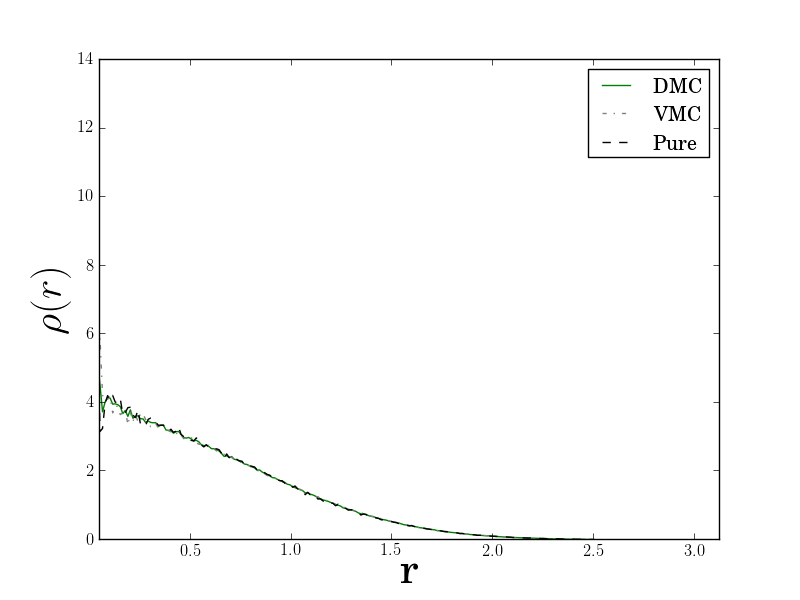
\includegraphics[scale=0.25]{../Graphics/OBD/OBD_Q3D/QD2w1_2D.png}} &
   \subfigure{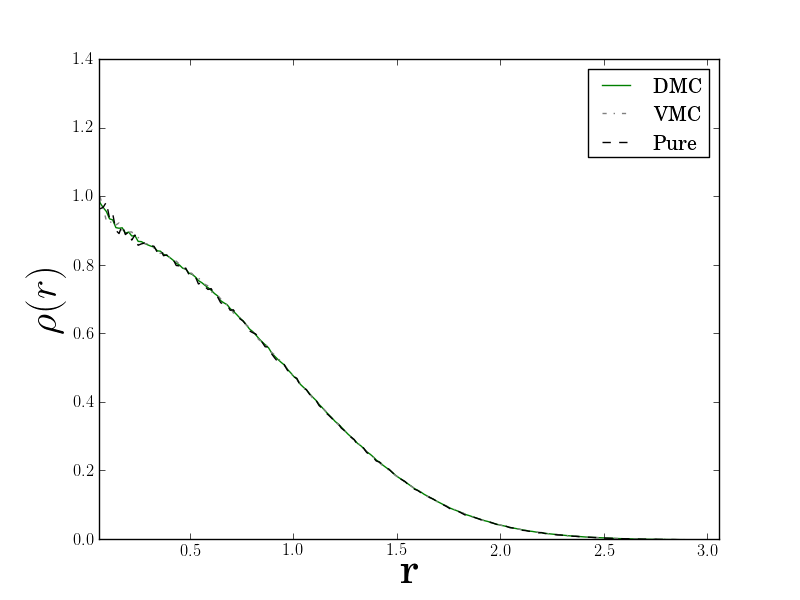
\includegraphics[scale=0.25]{../Graphics/OBD/OBD_Q3D/comp/Q2D_2.png}} \\
   \subfigure{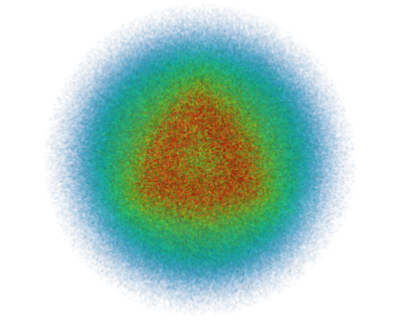
\includegraphics[scale=0.3]{../Graphics/OBD/OBD_Q3D/QD8w1_3D.png}} &
   \subfigure{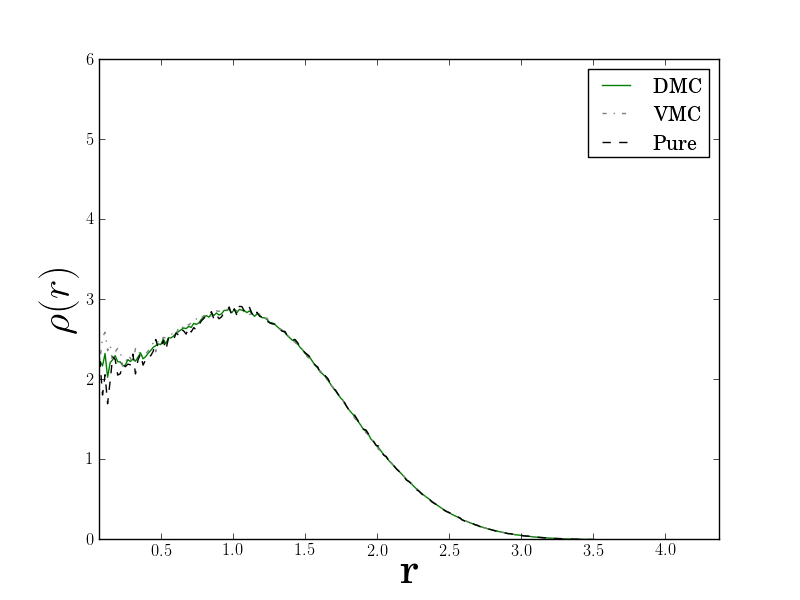
\includegraphics[scale=0.25]{../Graphics/OBD/OBD_Q3D/QD8w1_2D.png}} & 
   \subfigure{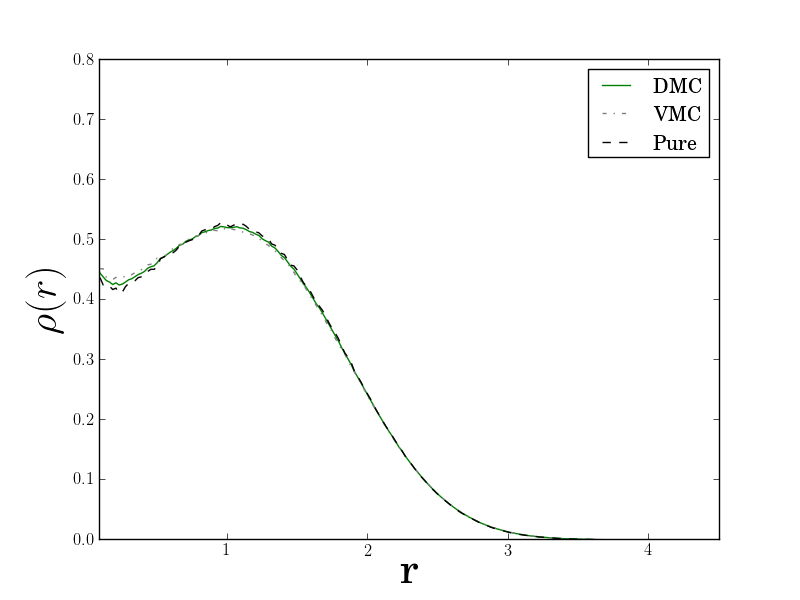
\includegraphics[scale=0.25]{../Graphics/OBD/OBD_Q3D/comp/Q2D_6.png}} \\
   \subfigure{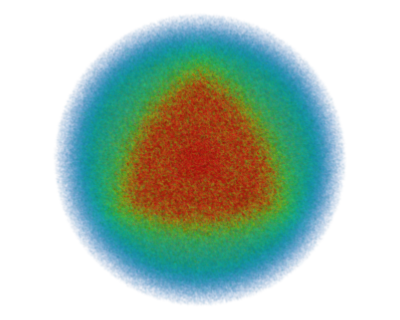
\includegraphics[scale=0.3]{../Graphics/OBD/OBD_Q3D/QD20w1_3D.png}} &
   \subfigure{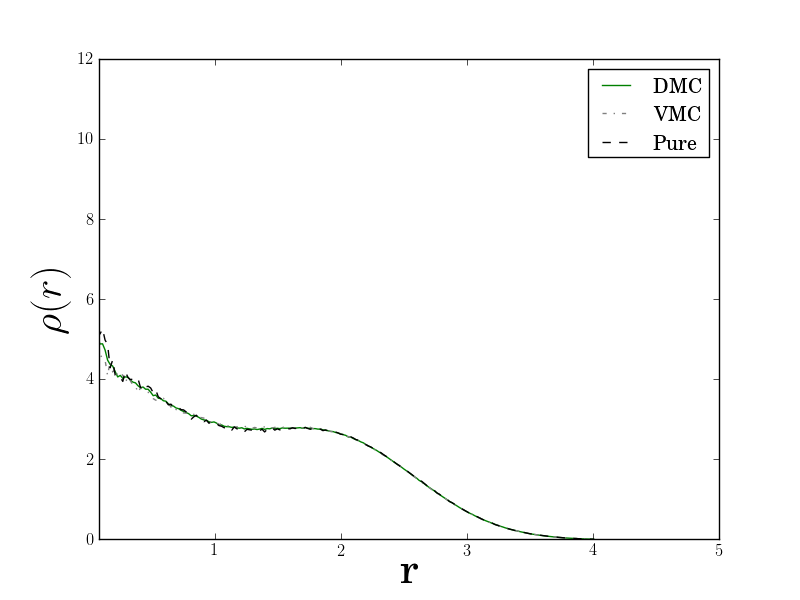
\includegraphics[scale=0.25]{../Graphics/OBD/OBD_Q3D/QD20w1_2D.png}} & 
   \subfigure{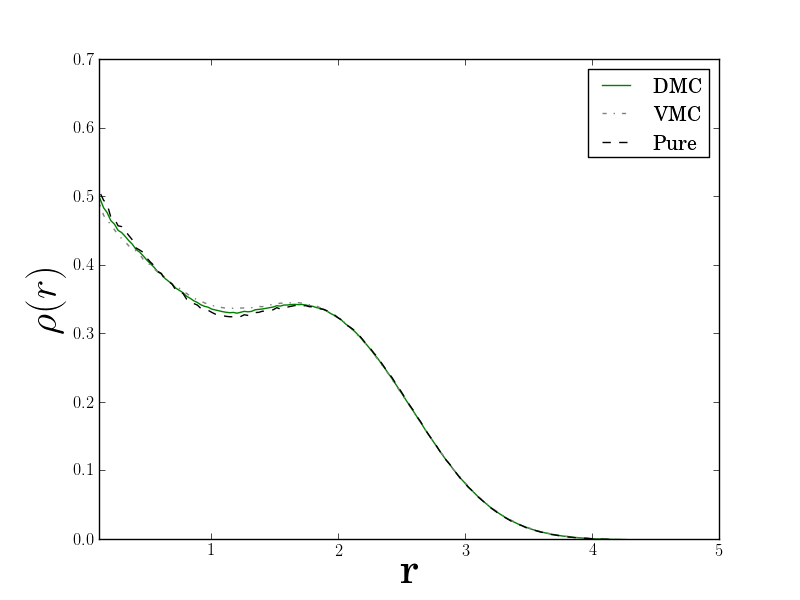
\includegraphics[scale=0.25]{../Graphics/OBD/OBD_Q3D/comp/Q2D_12.png}} \\
  \end{tabular}
  \caption{Left and middle column: One-body densities for quantum dots in three dimensions with frequency $\omega=1$. A quarter of the spherical density is removed to present a better view of the core. From top to bottom, the number of particles are $2$, $8$ and $20$ respectively. Right column: One-body densities for two dimensional quantum dots for $N=2$, $6$ and $12$ electrons with $\omega=1$. It is apparent that the  shape of the density is conserved as the third dimension is added. The difference is the number of particles a given structure can hold, i.e. a given shell. The radial densities are not normalized. Normalizing the densities would only change the vertical extent.}
  \label{fig:OBD_QDOTS3D_highfreq}
 \end{center}
\end{figure}
% \setlength{\tabcolsep}{pt}

\captionsetup[subfloat]{labelformat=parens}

\clearpage

\subsection{Lowering the frequency}


From Figure \ref{fig:OBD_QDOTS3D_lowfreq} it is apparent that lowering the frequency shifts the electrons away from the center of the potential. Moreover, Figure \ref{fig:OBD_DMC_QDOTS_lowering3D} reveals that the outer lying shells become just as populated as the inner lying shells, which means that all of the shells contain the same amount of particles on average.

This behavior is expected since the lower the frequency is set, the lower the energy cost of populating a higher shell becomes. 

An equally populated shell structure implies that it is not energetically efficient for the electrons to occupy several shells simultaneously, indicating that crystallization becomes the preferred positional state\footnote{Unless at least one particle is frozen in the QMC simulations, the Quantum Dot densities should always be rotationally symmetric. Crystallization in a QMC perspective comes thus not in the form of actual ``crystals'', but rather as a rotated crystallized state.}. This effect is called \textit{Wigner Crystallization}, and is expected for confined electrons where the correlation energy dominates the kinetic energy \textbf{cite wigner}. This effect has strong experimental evidence \textbf{cite wigner experiment}. 

The fact that the correlation energy dominates the kinetic energy is clear by looking at Figure \ref{fig:E_dist_qdots}. The kinetic energy contribution is almost constant with respect to the frequency, while the Coulomb energy contribution rapidly increases.

% \subsubsection{The critical limit}
% 
% Viewing the one-body densities for lower values of $\omega$ (Fig. \ref{fig:OBD_DMC_QDOTS_lowering3D}) in light of the corresponding densities for $\omega=1$ (Fig. \ref{fig:OBD_DMC_QDOTS_w1}), it is clear that there is little to no change in the density profile of $\omega=1$ to $\omega=0.28$. This is further verified by $\omega=0.5$ densities (not presented). 
% 
% This implies that the oscillator frequency merely scales the extent of the wave function and leaves the general density profile unchanged. However, going below $\omega=0.28$ reveals an interesting scenario where all of a sudden the densities change form. This is illustrated in figure \ref{fig:OBD_collapsed_w001}: At $\omega=0.1$ the changes become visible, yet the density is still comparable with that of higher frequencies. Going further down to $\omega=0.01$, the profile is entirely different, and will not collapse onto high frequency densities.
% 
% 
% 
% The frequency $\omega=0.28$ are used in numerous studies of Quantum Dots \textbf{referer}. The results of this section serve as a demonstration of why this apparently random limit is so widely applied; it is beyond this limit where the well-behaving high-frequency density profile starts to break down, leaving iterating methods struggling to converge. 
% 
% 
% 
% Lowering the frequency further, to $\omega=0.01$, interesting turn of events are revealed: The density profile completely changes, hardly resembling figure \ref{fig:OBD_collapsed_w001}. The number of shells increase due to the dominating Coulomb interaction. Moreover, these shells appear equally populated, if not more populated further out. This is the reversed effect than in the high-frequency case.
% 
% The ground state density represents the most energy efficient state of the particles given a potential, and it is therefore implied that the sudden change in the density profile at lower frequencies must be induced by a shift in the system's priorities between the different potential sources. In the case of Quantum Dots, these sources are the oscillator well and the Coulomb interaction. The amount of kinetic energy is also of interest.
% 
% It is tempting to state that the impact of the oscillator potential goes down proportional to the frequency squared (remember $V(\vec r) = \frac{1}{2}\omega^2r^2$), however, this view is in fact too naive, as the Coulomb interaction and the kinetic energy is dependent of the distribution of particles which in turn is dependent on the oscillator frequency. What is true, however, is that in the limit $\omega\to 0$, the effect of the oscillator potential is gone. 
% 
% Imagine an extremely narrow oscillator well: All the particles would favor stacking up in the center, as $r^2$ (oscillator) decrease quicker than $r^{-1}$ (Coulomb) increase. For lower frequencies we have the different situation where the particles would favor being very far apart, since the coefficient $\omega^2$ scaling the oscillator is very small. However, at a certain level, there comes a point where climbing the well further would cause the oscillator energy to increase more than Coulomb decrease. In other words, there is a balance - the oscillator will impact the particles even at very small frequencies. This is illustrated in Fig.
% 
% The question then becomes: Why do we get a change in the distribution below $\omega=0.28$ if a balance is always present between the oscillator and Coulomb? The answer is 

% The radial one-body densities are collapsed onto each other in Fig. \ref{fig:OBD_collapsed_w001} showing this effect in more detail. From this figure it is apparent that the density profiles of Quantum Dots with frequencies from $\omega=0.28$ and upwards are if fact extremely equal. At lower frequencies, the outer-lying shells gets an increase in particle population, and thus shifts the shape of the wave function as well as the extent.

\newcommand{\qqq}{\qquad\qquad\qquad}
\newcommand{\qq}{\qquad\qquad}
\newcommand{\rot}[1]{\begin{sideways}#1\end{sideways}}
\setlength{\tabcolsep}{0.1pt}
\begin{figure}
 \begin{center}
 \begin{tabular}{rl}
%    \subfigure{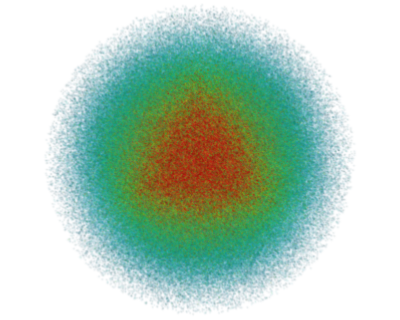
\includegraphics[scale=0.4]{../Graphics/OBD/OBD_Q3D/QD2w01_3D.png}} 
%    \subfigure{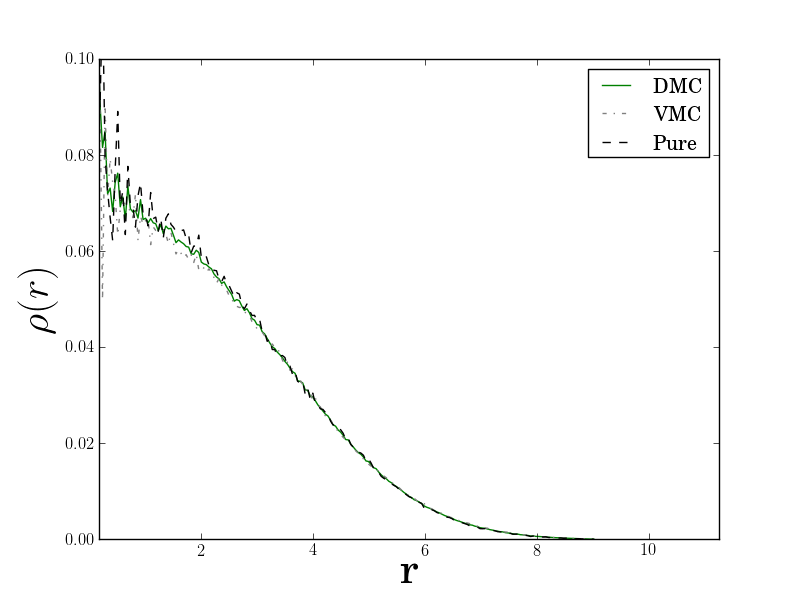
\includegraphics[scale=0.3]{../Graphics/OBD/OBD_Q3D/QD2w01_2D.png}}  \\
%    \subfigure{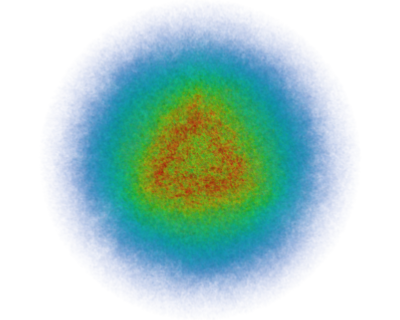
\includegraphics[scale=0.38]{../Graphics/OBD/OBD_Q3D/QD2w001_3D.png}} 
%    \subfigure{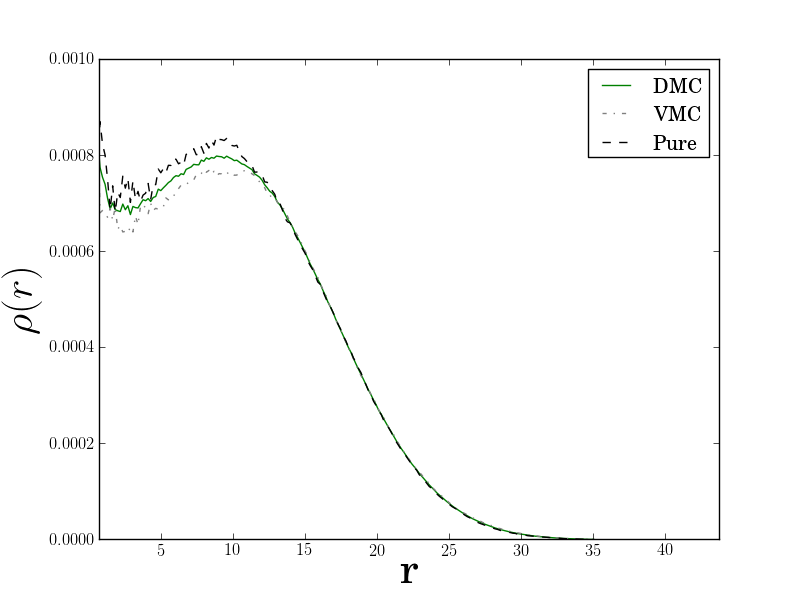
\includegraphics[scale=0.3]{../Graphics/OBD/OBD_Q3D/QD2w001_2D.png}}  \\
%    \subfigure{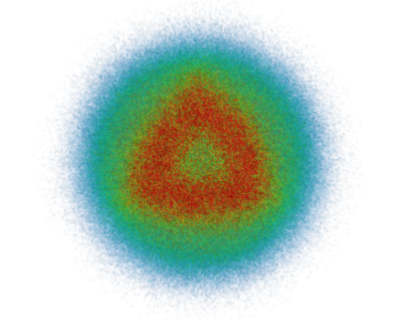
\includegraphics[scale=0.4]{../Graphics/OBD/OBD_Q3D/QD8w01_3D.png}} 
%    \subfigure{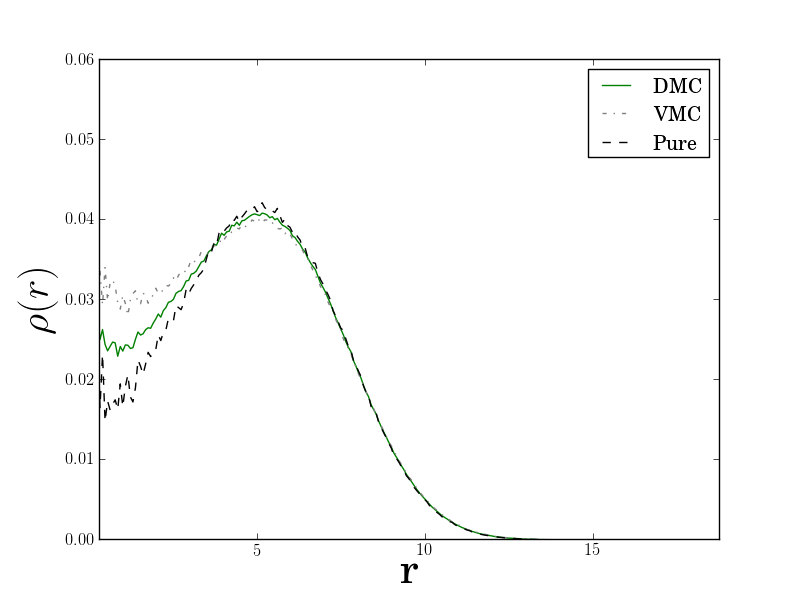
\includegraphics[scale=0.3]{../Graphics/OBD/OBD_Q3D/QD8w01_2D.png}}  \\
   \rot{$\qq\quad\omega=1$}&\subfigure{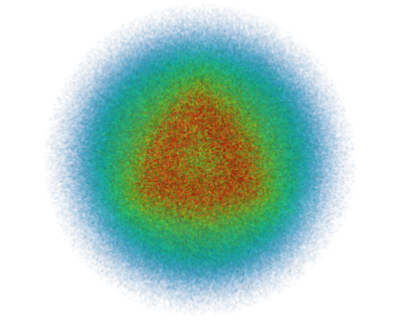
\includegraphics[scale=0.38]{../Graphics/OBD/OBD_Q3D/QD8w1_3D.png}}
   \subfigure{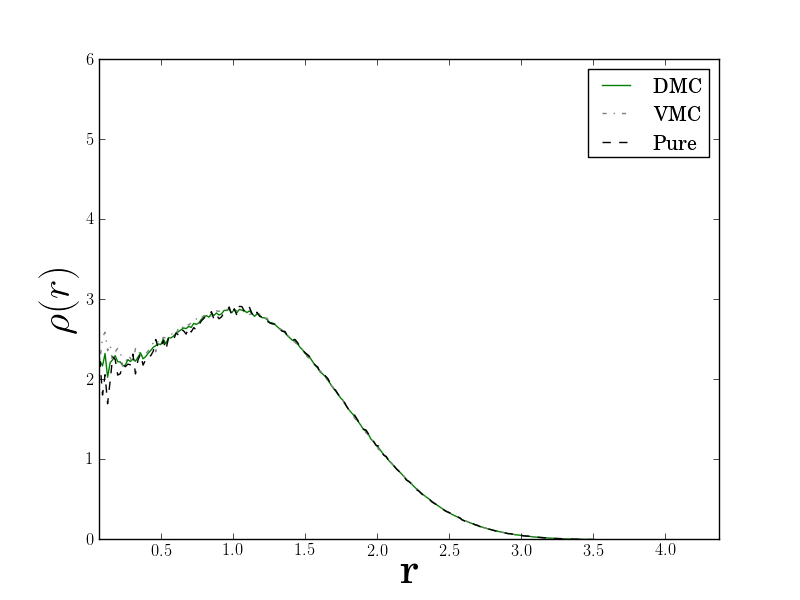
\includegraphics[scale=0.3]{../Graphics/OBD/OBD_Q3D/QD8w1_2D.png}} \\
   \rot{$\qq\omega=0.01$} &\subfigure{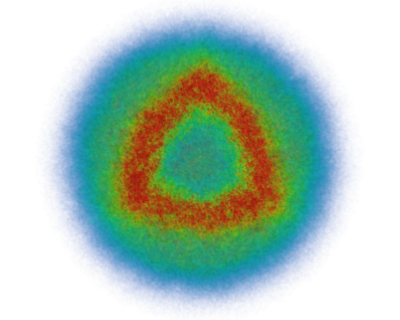
\includegraphics[scale=0.38]{../Graphics/OBD/OBD_Q3D/QD8w001_3D.png}} 
   \subfigure{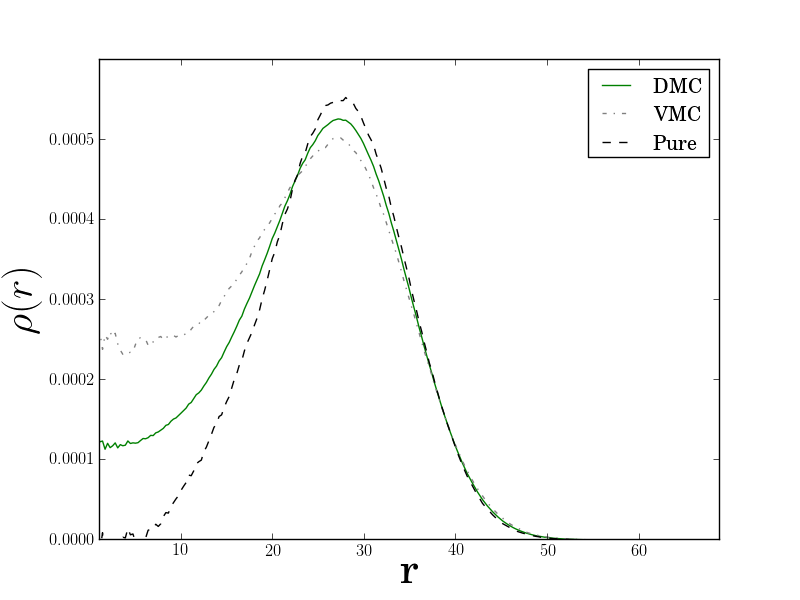
\includegraphics[scale=0.3]{../Graphics/OBD/OBD_Q3D/QD8w001_2D.png}}  \\
  \end{tabular}
  \caption{Comparison of the one-body densities for quantum dots in three dimensions for $N=8$ electrons for high and low frequency $\omega$. It is apparent that the distribution becomes more narrow as the frequency is reduced.}
  \label{fig:OBD_QDOTS3D_lowfreq}
 \end{center}
\end{figure}

\captionsetup[subfloat]{labelformat=empty}
\newcommand{\OBDscale}{0.25}
\begin{landscape}
 \begin{figure}
 \begin{center}
 \begin{tabular}{rl}
  \rot{$\qquad\quad\omega=0.28$}&\subfigure{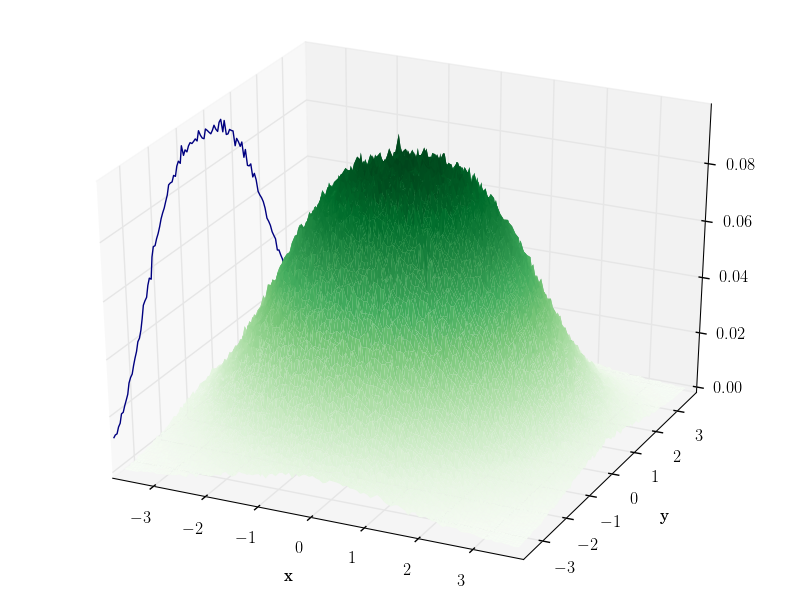
\includegraphics[scale=\OBDscale]{../Graphics/OBD/OBD_DMC/dist_out_QDots2c028_3D.png}}
  \subfigure{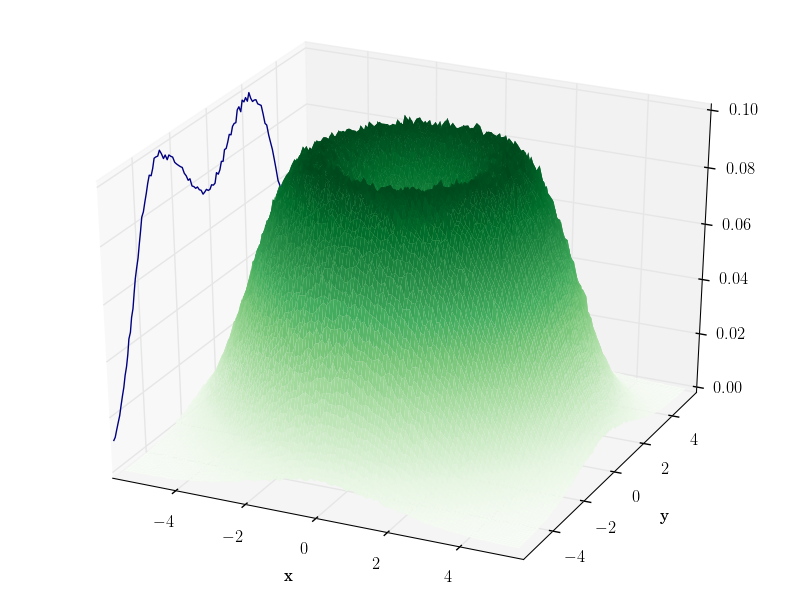
\includegraphics[scale=\OBDscale]{../Graphics/OBD/OBD_DMC/dist_out_QDots6c028_3D.png}} 
  \subfigure{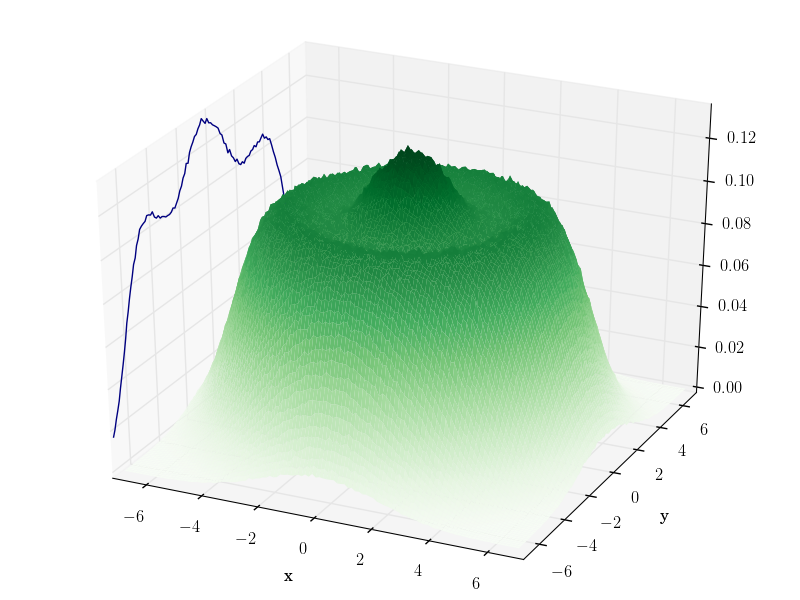
\includegraphics[scale=\OBDscale]{../Graphics/OBD/OBD_DMC/dist_out_QDots12c028_3D.png}}
  \subfigure{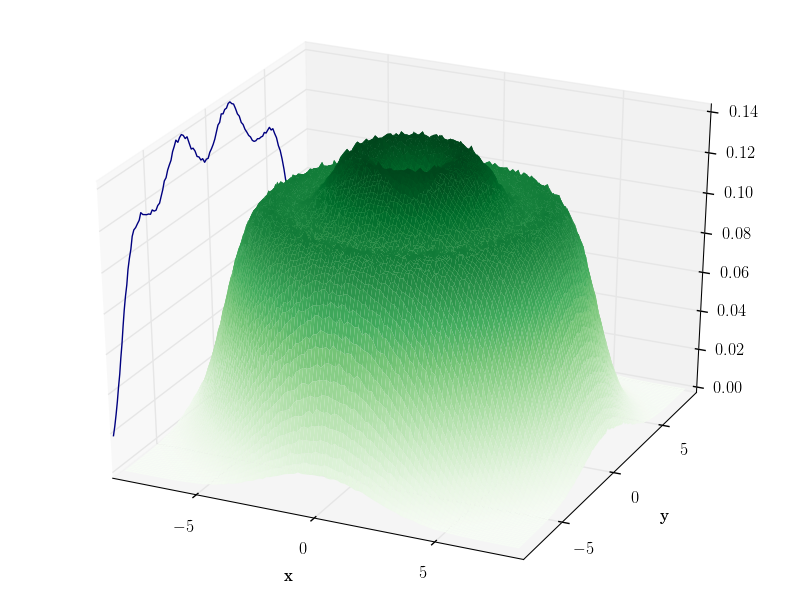
\includegraphics[scale=\OBDscale]{../Graphics/OBD/OBD_DMC/dist_out_QDots20c028_3D.png}} \\[-0pt]
  \rot{$\qquad\quad\omega=0.1$}&\subfigure{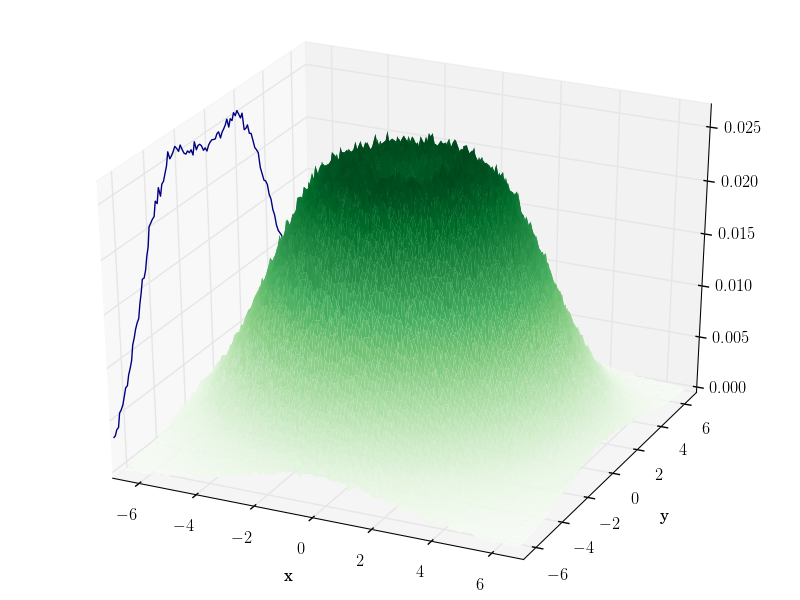
\includegraphics[scale=\OBDscale]{../Graphics/OBD/OBD_DMC/dist_out_QDots2c01_3D.png}}
  \subfigure{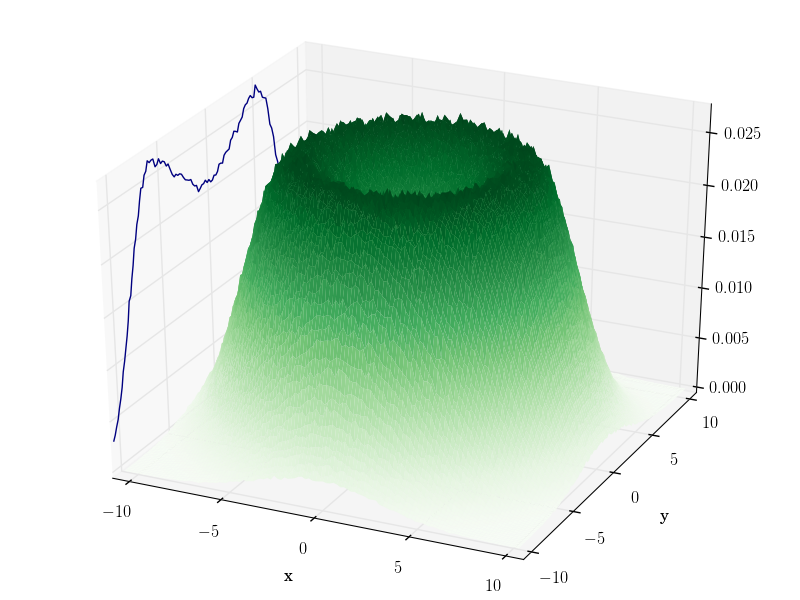
\includegraphics[scale=\OBDscale]{../Graphics/OBD/OBD_DMC/dist_out_QDots6c01_3D.png}} 
  \subfigure{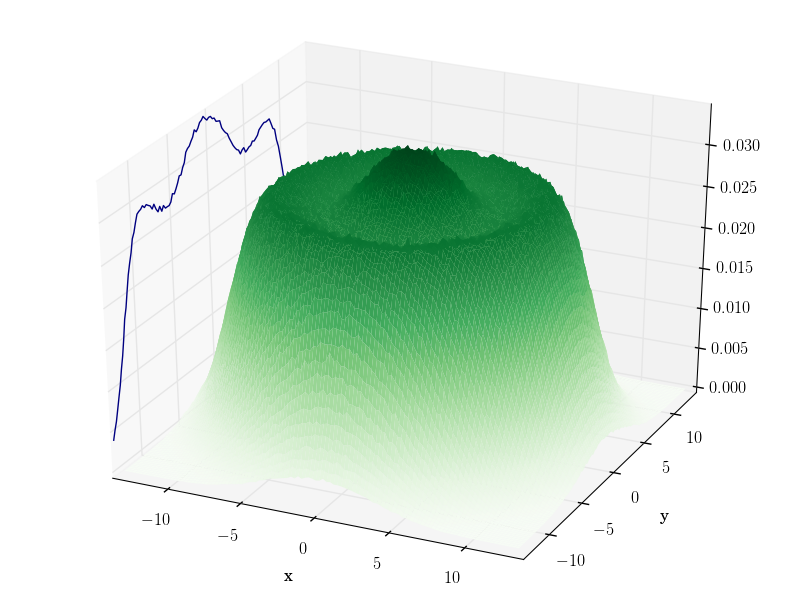
\includegraphics[scale=\OBDscale]{../Graphics/OBD/OBD_DMC/dist_out_QDots12c01_3D.png}}
  \subfigure{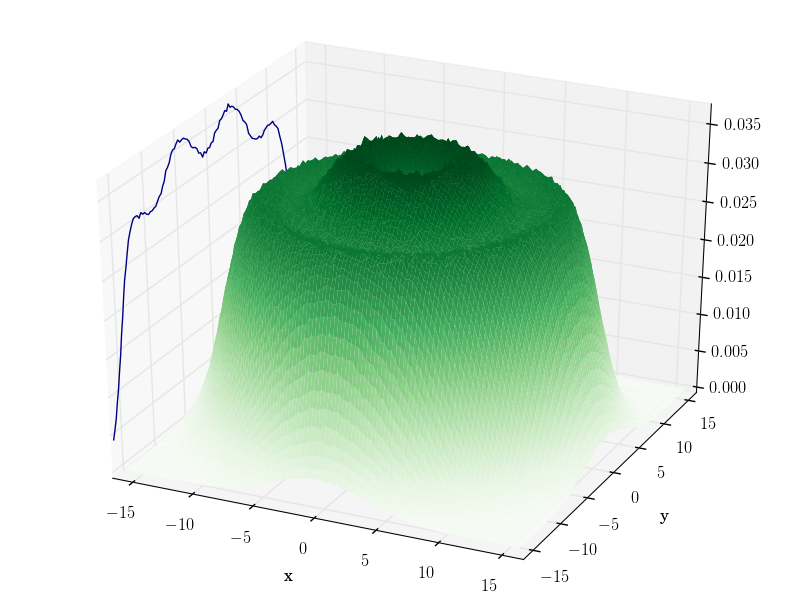
\includegraphics[scale=\OBDscale]{../Graphics/OBD/OBD_DMC/dist_out_QDots20c01_3D.png}} \\[-0pt]
  \rot{$\qquad\quad\omega=0.01$}&\subfigure[$N=2$]{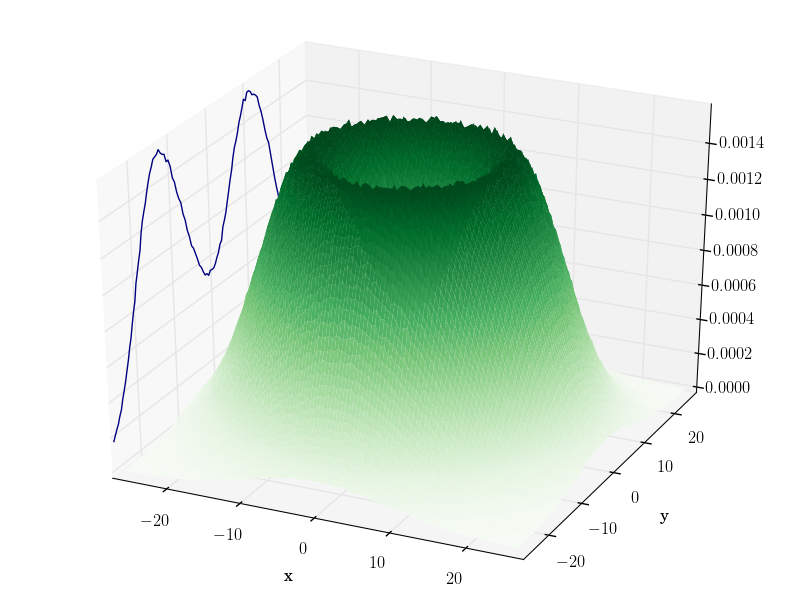
\includegraphics[scale=\OBDscale]{../Graphics/OBD/OBD_DMC/dist_out_QDots2c001_3D.png}}
  \subfigure[$N=6$]{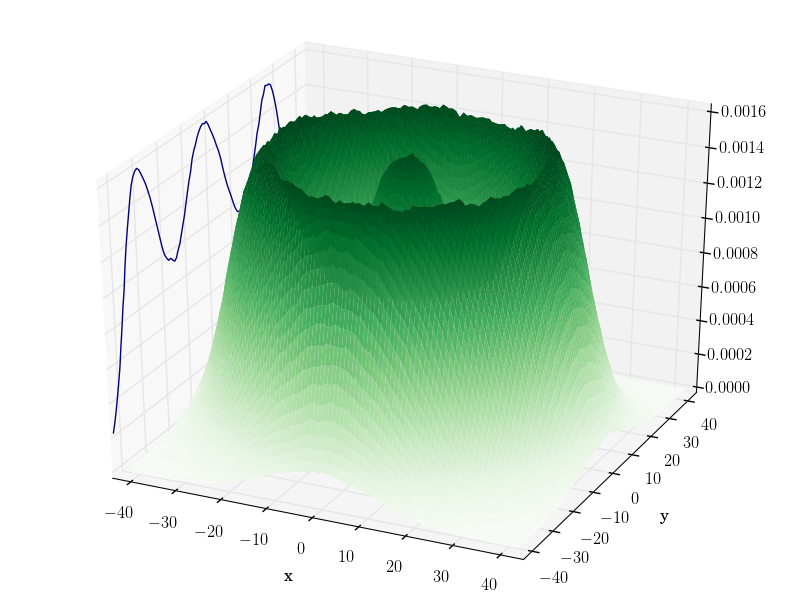
\includegraphics[scale=\OBDscale]{../Graphics/OBD/OBD_DMC/dist_out_QDots6c001_3D.png}} 
  \subfigure[$N=12$]{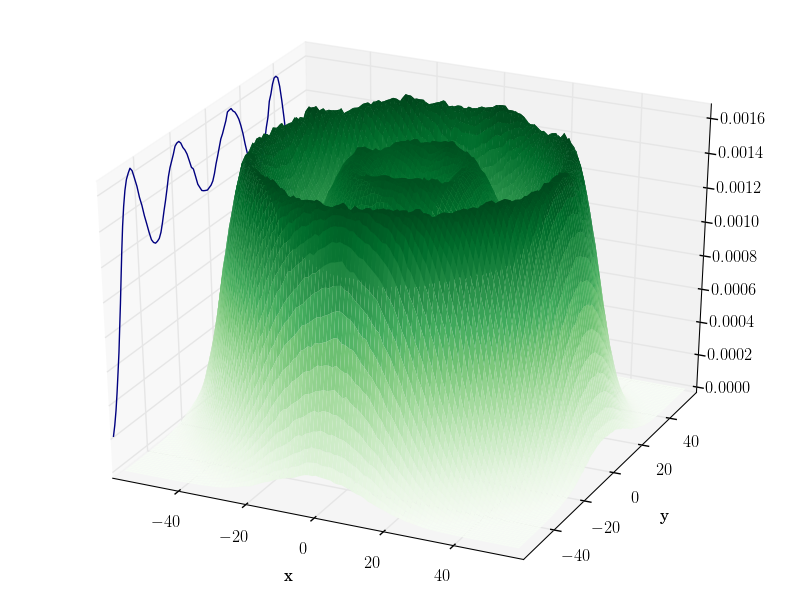
\includegraphics[scale=\OBDscale]{../Graphics/OBD/OBD_DMC/dist_out_QDots12c001_3D.png}}
  \subfigure[$N=20$]{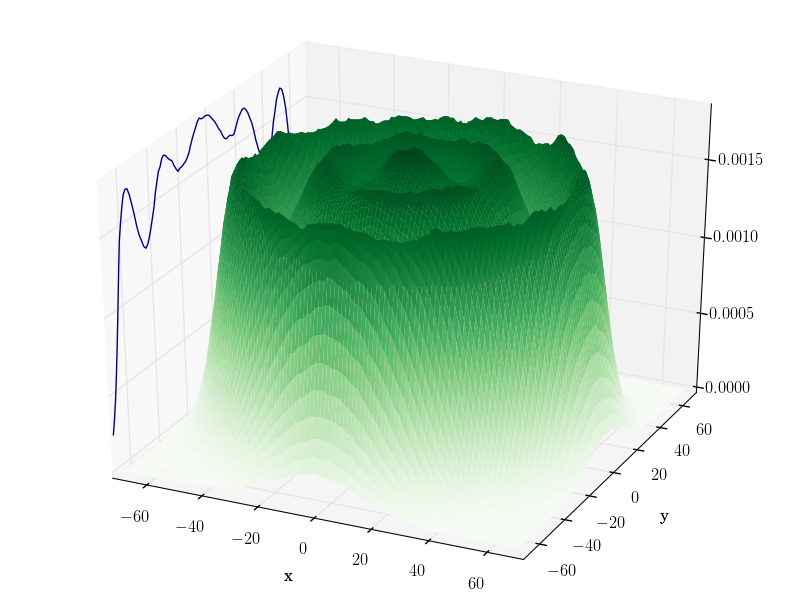
\includegraphics[scale=\OBDscale]{../Graphics/OBD/OBD_DMC/dist_out_QDots20c001_3D.png}} \\
 \end{tabular}
  \caption{\small{DMC One-body densities for Quantum Dots for decreasing oscillator frequencies $\omega$ and increasing number of particles $N$. Each row represents a given $\omega$, and each column represents a given $N$. Notice that the densities for $\omega=1$ (from figure \ref{fig:OBD_DMC_QDOTS_w1}) are indistinguishable from those of $\omega=0.28$ except for their radial extent. This trend has been verified in the case of $N=30$, 42 and 56 electrons as well as for $\omega=0.5$, however, for the sake of transparency, these results are left out of the current figure. Results for $N=30$, 42 and 56 particles for $\omega=0.01$ has too wide radial extent to converge with the computational resources available at the present time and has thus not been computed.}}
  \label{fig:OBD_DMC_QDOTS_lowering3D}
 \end{center}
\end{figure}
\end{landscape}

\captionsetup[subfloat]{labelformat=parens}
\setlength{\tabcolsep}{6pt}


% \clearpage
% 
% \newcommand{\OBDscaleR}{0.3}
% \setlength{\tabcolsep}{5pt}
% \captionsetup[subfloat]{labelformat=empty}
% \begin{figure}
%  \begin{center}
%  \begin{tabular}{lr}
%    \rot{$\qqq N=2$}  & \subfigure{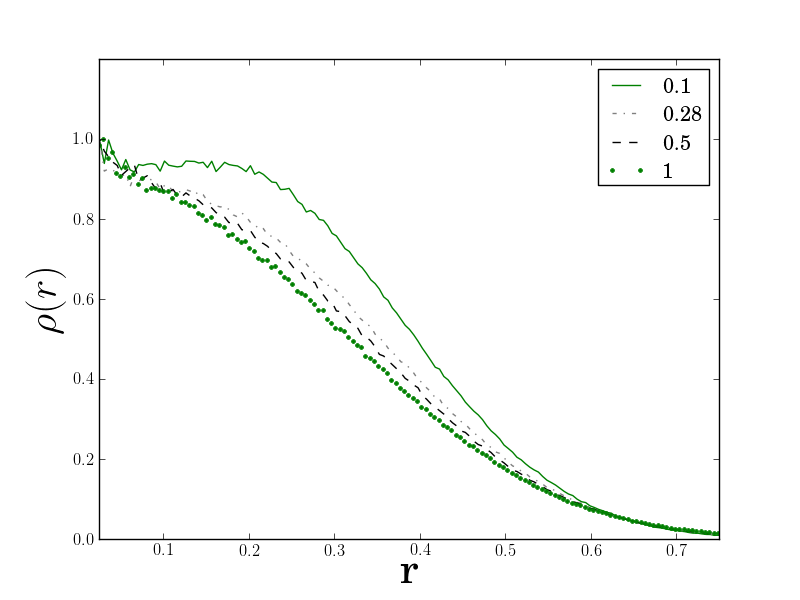
\includegraphics[scale=\OBDscaleR ]{../Graphics/OBD/OBD_rad_psort/QDots_2.png}} 
%   \subfigure{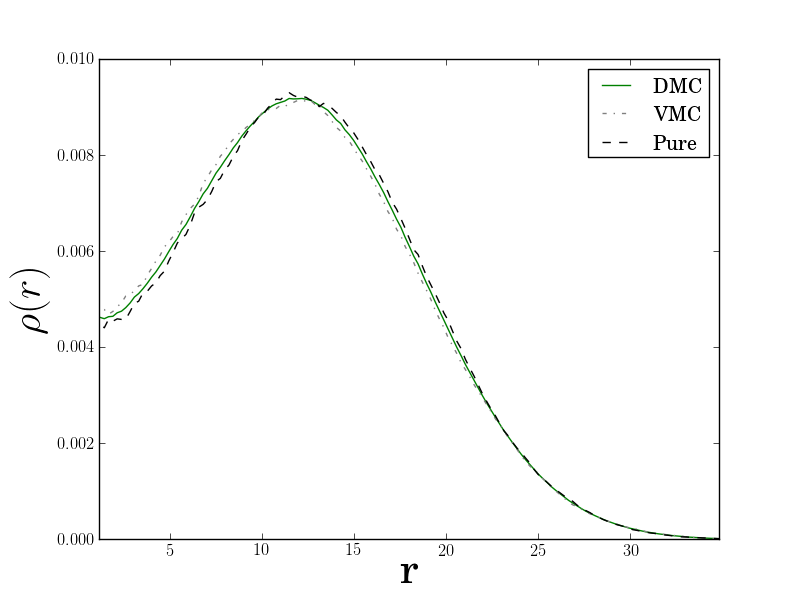
\includegraphics[scale=\OBDscaleR ]{../Graphics/OBD/OBD_w001/QDots_2.png}} \\[-0pt]
%    \rot{$\qqq N=6$}  & \subfigure{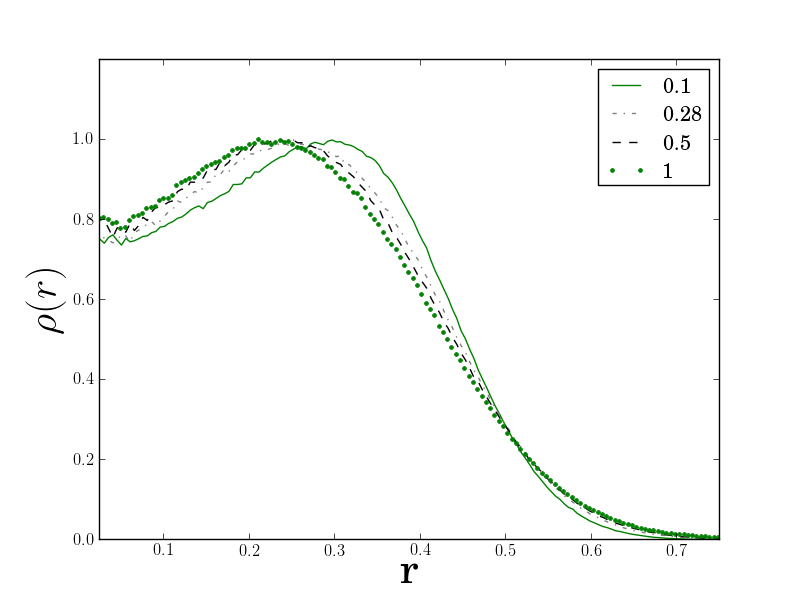
\includegraphics[scale=\OBDscaleR]{../Graphics/OBD/OBD_rad_psort/QDots_6.png}}
%   \subfigure{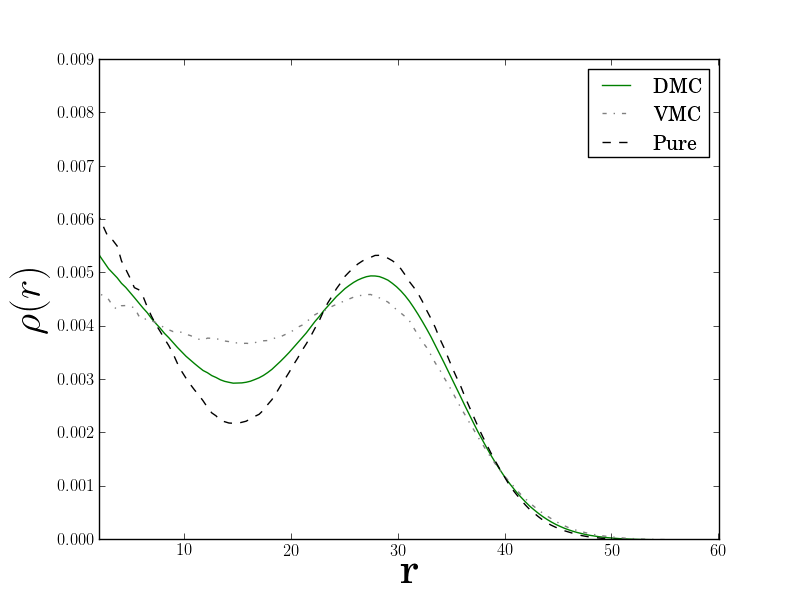
\includegraphics[scale=\OBDscaleR ]{../Graphics/OBD/OBD_w001/QDots_6.png}} \\[-0pt]
%    \rot{$\qqq N=12$} & \subfigure{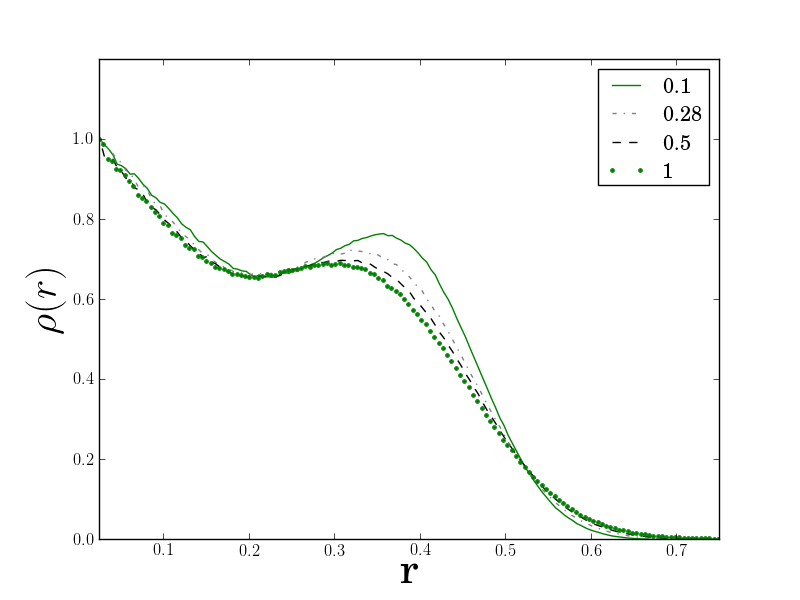
\includegraphics[scale=\OBDscaleR]{../Graphics/OBD/OBD_rad_psort/QDots_12.png}} 
%   \subfigure{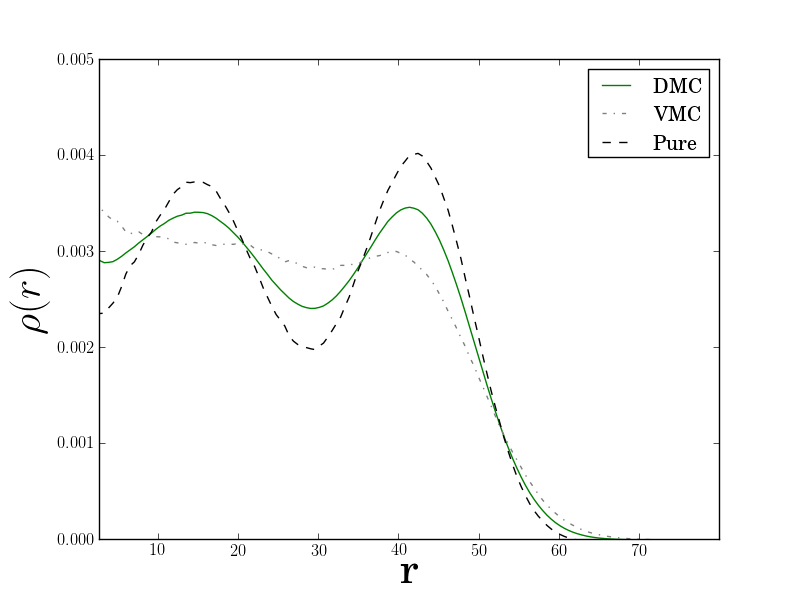
\includegraphics[scale=\OBDscaleR ]{../Graphics/OBD/OBD_w001/QDots_12.png}} \\[-0pt]
%    \rot{$\qqq N=20$} & \subfigure[Collapsed results]{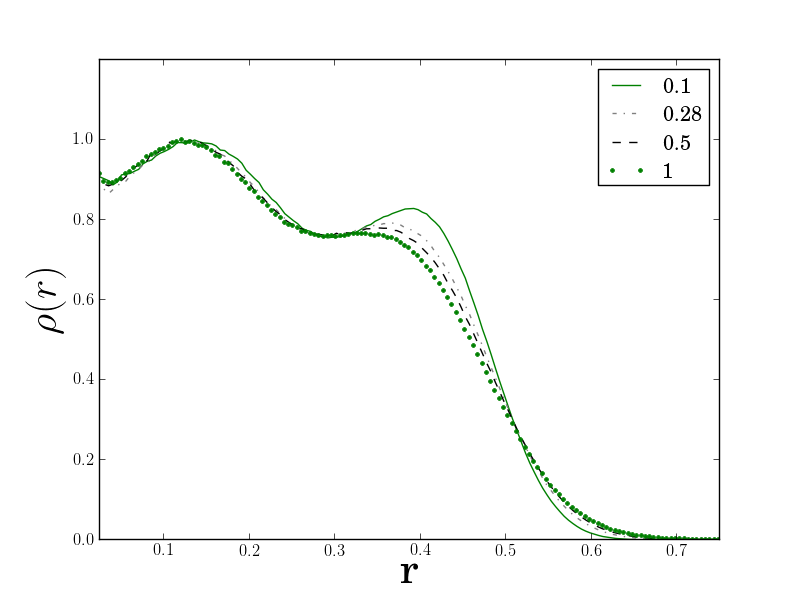
\includegraphics[scale=\OBDscaleR]{../Graphics/OBD/OBD_rad_psort/QDots_20.png}}
%   \subfigure[$\omega=0.01$]{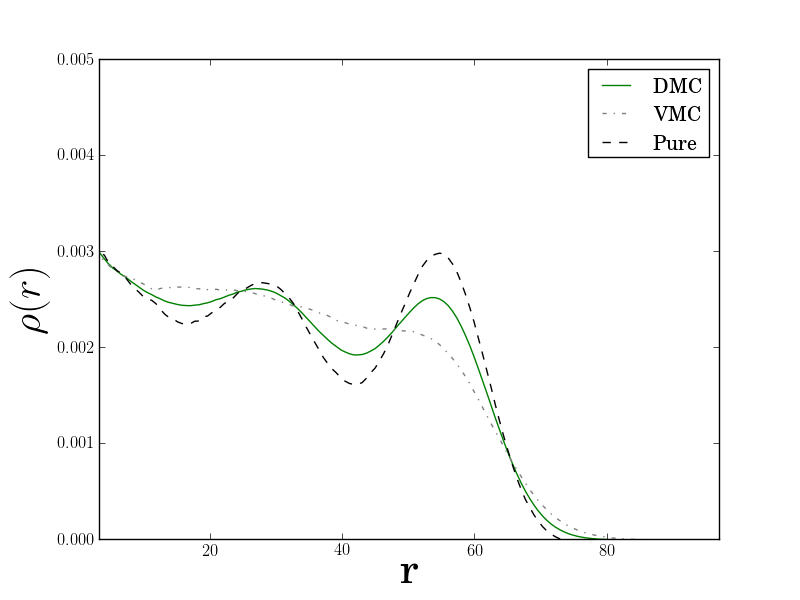
\includegraphics[scale=\OBDscaleR]{../Graphics/OBD/OBD_w001/QDots_20.png}} \\[-0pt]
%   \end{tabular}
%   \caption{Right column: Radial one-body densities for high frequencies (see specific legends). Left column: Radial one-body densities for $\omega=0.01$.}
%   \label{fig:OBD_collapsed_w001}
%  \end{center}
% \end{figure}
% \setlength{\tabcolsep}{6pt}
% \captionsetup[subfloat]{labelformat=parens}
% \clearpage

% 
% \captionsetup[subfloat]{labelformat=empty}
% \begin{figure}
%  \begin{center}
%   \subfigure[$N=2$]{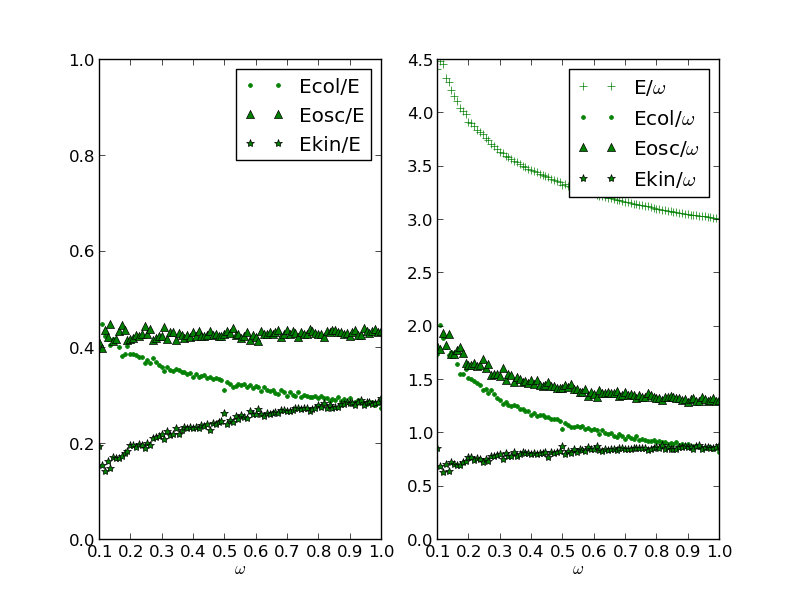
\includegraphics[scale=0.35]{../Graphics/VirialPlots/E_vs_w_E2.png}}
%   \subfigure[$N=6$]{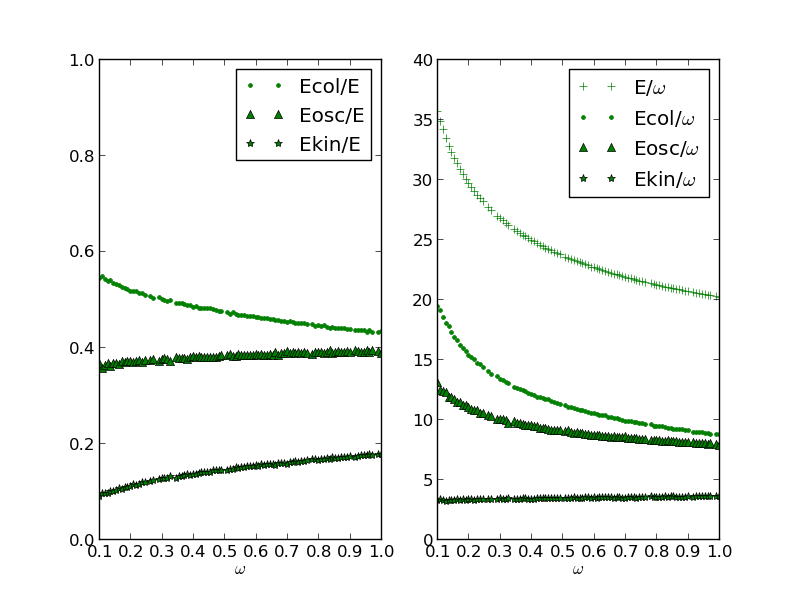
\includegraphics[scale=0.35]{../Graphics/VirialPlots/E_vs_w_E6.png}} \\
%   \subfigure[$N=12$]{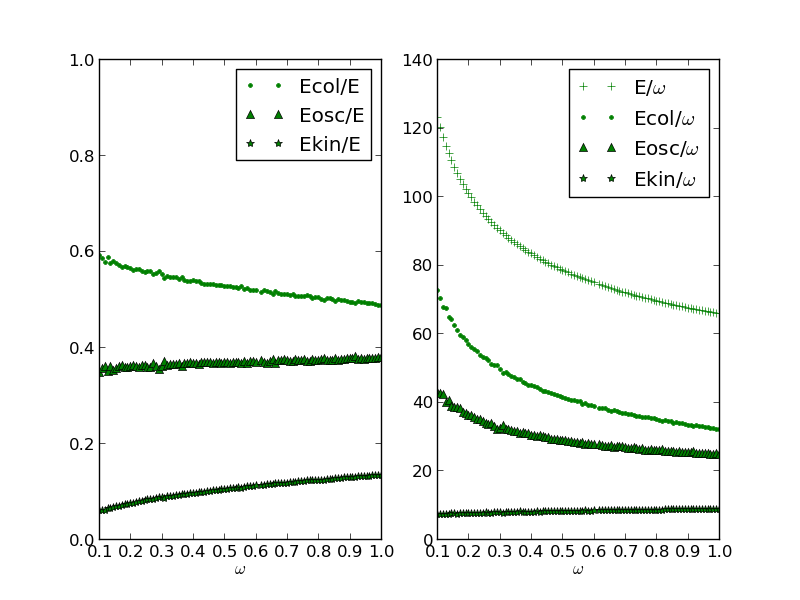
\includegraphics[scale=0.35]{../Graphics/VirialPlots/E_vs_w_E12.png}}
%   \subfigure[$N=20$]{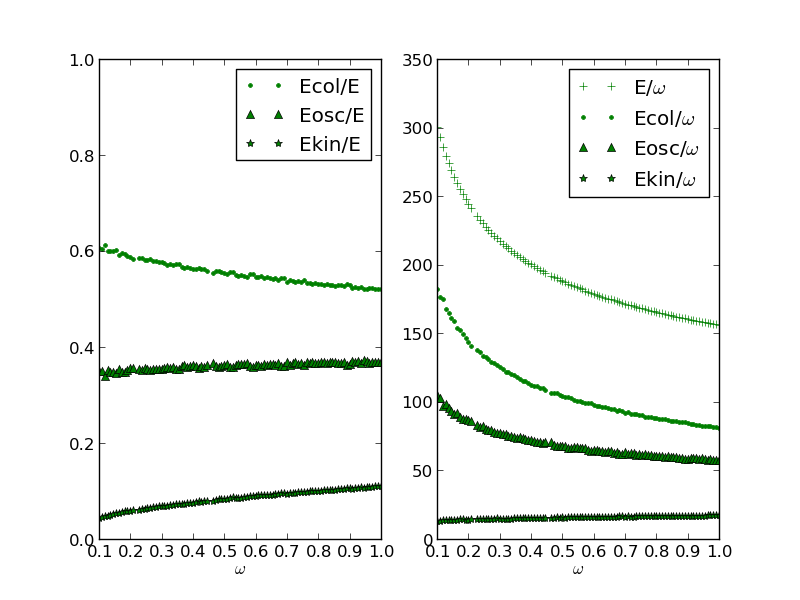
\includegraphics[scale=0.35]{../Graphics/VirialPlots/E_vs_w_E20.png}} \\
%   \subfigure[$N=30$]{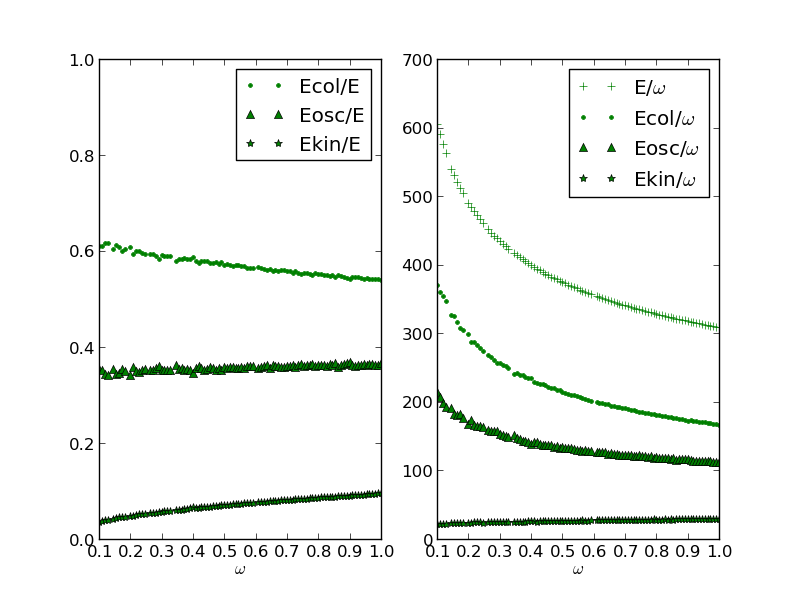
\includegraphics[scale=0.35]{../Graphics/VirialPlots/E_vs_w_E30.png}}
%   \subfigure[$N=42$]{\includegraphics[scale=0.35]{../Graphics/VirialPlots/E_vs_w_E42.png}} \\
%   \caption{}
%   \label{fig:E_dist_qdots}	
%  \end{center}
% \end{figure}
% 
% \begin{figure}
%  \begin{center}
%   \subfigure[$N=2$]{\includegraphics[scale=0.35]{../Graphics/VirialPlots/E_vs_w_V2.png}}
%   \subfigure[$N=6$]{\includegraphics[scale=0.35]{../Graphics/VirialPlots/E_vs_w_V6.png}} \\
%   \subfigure[$N=12$]{\includegraphics[scale=0.35]{../Graphics/VirialPlots/E_vs_w_V12.png}}
%   \subfigure[$N=20$]{\includegraphics[scale=0.35]{../Graphics/VirialPlots/E_vs_w_V20.png}} \\
%   \subfigure[$N=30$]{\includegraphics[scale=0.35]{../Graphics/VirialPlots/E_vs_w_V30.png}}
%   \subfigure[$N=42$]{\includegraphics[scale=0.35]{../Graphics/VirialPlots/E_vs_w_V42.png}} \\
%   \caption{}
%   \label{fig:V_dist_qdots}
%  \end{center}
% \end{figure}
% \captionsetup[subfloat]{labelformat=parens}


\captionsetup[subfloat]{labelformat=empty}
\begin{figure}[h]
 \begin{center}
  \subfigure[$N=6$]{\includegraphics[scale=0.35]{../Graphics/VirialPlots/E_vs_w_E6.png}}
  \subfigure[$N=42$]{\includegraphics[scale=0.35]{../Graphics/VirialPlots/E_vs_w_E42.png}} \\
  \caption{The relative magnitude of the different energy sources as a function of the frequency $\omega$ (left) together with the magnitude of the sources' energy contributions scaled with the oscillator frequency (right). The plots are supplied with legends to increase the readability. The different energy sources are kinetic (kin), oscillator (osc) and Coulomb (col). It is apparent that the kinetic contribution is constant in both cases and the potential contribution is constant for the relative energies. The values are calculated using two dimensional quantum dots. The number of electrons $N$ are displayed beneath each respective plot.}
  \label{fig:E_dist_qdots}
 \end{center}
\end{figure}

In other words, quantum dots fall into a crystallized state at low frequencies. In light of the previous discussion regarding Wigner crystallization, this follows as a consequence of the kinetic energy being dominated by the Coulomb energy. Since the Coulomb energy in turn dominates the oscillator energy (the left-hand side parts of the plots in Figure \ref{fig:E_dist_qdots}), the interesting quantity to study is the kinetic energy as a function of the total potential energy. 

This is closely related to the \textit{virial theorem} from classical mechanics. The quantum mechanical version of the virial theorem was proven by Fock in 1930 \cite{} and reads

\begin{equation}
 V(\mathbf{r}) \propto r^\gamma \quad\longrightarrow\quad \langle \OP{T} \rangle = \frac{\gamma}{2} \langle \OP{V} \rangle, \label{eq:virial}
\end{equation}

where $\OP{T}$ and $\OP{V}$ denote the kinetic - and potential energy operators respectively. The important conclusion which can be drawn from this is that a constant slope in the kinetic - vs. potential energy plot implies that the systems behave identically, that is, they follow the same effective potential and thus have similar eigenstates. From Figure \ref{fig:V_dist_qdots} it is apparent that there is a remarkably constant slope for two different regions: High - and low kinetic energy, which by looking at Figure \ref{fig:E_dist_qdots} corresponds to high - and low frequencies. This proves that the system changes characteristics as the frequency changes, which explains the sudden change in the density profiles.



\newpage

\begin{figure}[h]
 \begin{center}
  \subfigure[$N=6$]{\includegraphics[scale=0.35]{../Graphics/VirialPlots/E_vs_w_V6.png}}
  \subfigure[$N=42$]{\includegraphics[scale=0.35]{../Graphics/VirialPlots/E_vs_w_V42.png}} \\
  \caption{The total kinetic energy vs. the total potential energy of two dimensional quantum dots. The number of electrons $N$ are displayed beneath each respective plot. The axes are scaled with a power of $N$ to collapse the data to the same axis span. Once the kinetic energy drops below a certain energy dependent on the number of particles, the slope changes, which in light of the virial theorem from Eq.~(\ref{eq:virial}) indicates that the overall system changes properties. The data is fitted with linear lines with slopes $a$. The parameter $r2$ indicates how well the data fits a linear line, and is exact in the case of $r2 = 1$.}
  \label{fig:V_dist_qdots}
 \end{center}
\end{figure}
\captionsetup[subfloat]{labelformat=parens}

\subsection{Simulatings in a Double-well}

awesome